\chapter{Geodesics on surfaces}\label{chapter:geodesics}%
\chapterSummary{%
Geodesics are locally shortest paths on a surface.
We prove that they exist and that they are smooth.}

\section{Geodesic flow}
Each point \(\pr{x^o,e^o} \in \frameBundleE{3}\) moves along a path \(x(t)=x^o + t e^o_1, e(t)=e^o\).
In other words, don't rotate the frame, but slide the base point \(x\) along the direction of the first leg of the frame.
\begin{center}
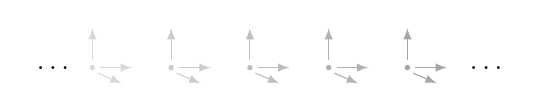
\begin{tikzpicture}
\node at (2.5,0) {\(\dots\)};
\foreach \i in {30,40,...,70}{
  \fill [fill={gray!\i!white}] ({.1*\i},0) circle (1pt);% node[above];%{\(x\)};
  \draw[-latex,draw={gray!\i!white},fill={gray!\i!white}] ({.1+.1*\i},0) -- ({.5+.1*\i},0);% node[below left];%{\(e_1\)};
  \draw[-latex,draw={gray!\i!white},fill={gray!\i!white}] ({.1*\i},.1) -- ({.1*\i},.5);% node[below right];%{\(e_2\)};
  \draw[-latex,draw={gray!\i!white},fill={gray!\i!white}] ({.07+.1*\i},-.07) -- ({.07+.1*\i+.3},{-.2});% node[below right];%{\(e_2\)};
  }
\node at (8,0) {\(\dots\)};
\end{tikzpicture}
\end{center}
\par\noindent{}%
Define a vector field \(\geodesicVectorField(x,e)\defeq\pr{e_1,0}\) on \(\frameBundleE{3}\);  these paths are its flow lines.

Imitate this vector field on the frame bundle of a surface \(S\) in \(\E[3]\).
Write points of \(\frameBundle{S} \times \E[2]\) as \(\pr{x,e,y}\) for \(y \in \E[2]\).
The \emph{geodesic spray}\define{geodesic!spray}\define{spray!geodesic} of \(S\) is  the vector field \(\geodesicVectorField\) on \(\frameBundle{S} \times \E[2]\) given by
\[
\geodesicVectorField \hook \pr{\omega,\alpha,dy}=\pr{y,0,0}
\]
This expression does \emph{not} involve \(\gamma_{13}\) or \(\gamma_{23}\), since these are not linearly independent \(1\)-forms on \(\frameBundle{S}\).
The flow of \(\geodesicVectorField\) is the \emph{geodesic flow}.%
\define{flow, geodesic}\define{geodesic!flow}
The vector field \(\geodesicVectorField\) moves every frame \(\pr{x,e}\), moving \(x\) in the direction of \(\sum y_i e_i\), and ``not rotating'' the frame \(e\), since \(\geodesicVectorField \hook \gamma_{12}=0\).
Intuitively, \(\geodesicVectorField\) twists frames only in the normal directions (in the \(\gamma_{13}, \gamma_{23}\) directions), not tangentially (the \(\alpha=\gamma_{12}\) direction), while keeping \(e_1,e_2\) tangent to the surface \(S\).
Map \(\pr{x,e} \in \frameBundle{S} \to \pr{x,e,(1,0)} \in \frameBundle{S} \times \E[2]\), so that \(\frameBundle{S}\) is identified with a submanifold of \(\frameBundle{S} \times \E[2]\), making \(\frameBundle{S}\) invariant under the geodesic flow.
Write \(\transpose{a}\) for the transpose of a matrix \(a\).
Let \(g \in \Orth{2} \times \pm 1\) act on \(\frameBundle{S}\times\E[2]\) by
\[
(x,e,y)g=(x,eg,\transpose{a} y).
\]
if
\[
g = \begin{pmatrix}
        a & 0 \\
        0 & b
       \end{pmatrix}.
\]

\begin{lemma}
On \(\frameBundle{S} \times \E[2]\), \(r^*_g \pr{\omega,\gamma_{12},dy}=\pr{\transpose{g} \omega, \gamma_{12}, \transpose{g} \, dy}\) while \(r_{g*} \geodesicVectorField=\geodesicVectorField\).
\end{lemma}
\begin{proof}
The reader can check how the \(1\)-forms pull back.
The equations defining \(\geodesicVectorField\) imply invariance under \(\Orth{2} \times \pm 1\).
\end{proof}

Let \(p \colon (x,e,y) \in \frameBundle{S} \times \E[2] \mapsto (x,v) \in TS\) by \(v=\sum y_i e_i\).

\begin{proposition}
There is a uniquely determined vector field \(\geodesicVectorField\) on \(TS\), also called the \emph{geodesic spray}, so that \(p_* \geodesicVectorField = \geodesicVectorField\).
\end{proposition}
\begin{proof}
Calculate that at a point \(z=(x,e,y)\), for any \(g \in \Orth{2} \times \pm 1\),
\begin{align*}
p'(zg) \geodesicVectorField(zg)
&=
p'(zg) r_g'(z) \geodesicVectorField(z),
\\
&=
\pr{p \circ r_g}'(z) \geodesicVectorField(z), 
\\
&=
p'(z) \geodesicVectorField(z).
\end{align*}
The reader can check that \(\Orth{2} \times \pm 1\) acts transitively on the points \(z=(x,e,y)\) lying above a given point \((x,v)=p(z)\).
Therefore the vector \(p'(z) \geodesicVectorField(z)\) is independent of the point \(z\), depending only on \((x,v)=p(z)\). 
\end{proof}

A \emph{geodesic}%
\define{geodesic}
is a curve in \(S\) which is a projection to \(S\) of a flow line of \(\geodesicVectorField\) in \(TS\).


\begin{problem}{moving.frame:geods}
Take a surface \(S\) in \(\E[3]\).
Prove that any geodesic \(x(t)\) of \(S\), as a curve in \(\E[3]\), has geodesic curvature \(a\of{\dot{x},\dot{x}}\).
Prove that \(a=0\) just when all geodesics of \(S\) are geodesics of \(\E[3]\), i.e. straight lines, so that \(S\) is locally an open subset of a plane.
\end{problem}


\begin{lemma}
A smooth curve \(C\) on a surface \(S\) in \(\E[3]\) has vanishing geodesic curvature just when it is a geodesic.
\end{lemma}
\begin{proof}
The geodesic spray vector field \(\geodesicVectorField\) points along the tangent line cut out by the equations \(\omega_2=0\) and \(\alpha=0\) and has \(\geodesicVectorField \hook \omega_1=1\).
The tangent spaces of \(\adaptedFrameBundle{C}{S}\) are cut out by the equations \(\omega_2=0\) and \(\alpha=-\kappa_2 \omega_1\).
The geodesic spray \(\geodesicVectorField\) lies tangent to \(\adaptedFrameBundle{C}{S}\) just when the geodesic curvature of \(C\) vanishes, which therefore occurs just when the projection of the flow lines of \(\geodesicVectorField\) lie along \(C\), i.e. \(C\) is a geodesic.
\end{proof}


\section{First order deformation}
Take a plane curve \(\pr{x(s),y(s)}\in\R[2]\).
Draw a vector field along this curve: a vector \(\pr{u(s),v(s)}\) at each point \(\pr{x(s),y(s)}\).
The smooth homotopy \(s,t \mapsto \pr{x(s)+tu(s),y(s)+tv(s)}\) pushes out each point \(\pr{x(s),y(s)}\) in the direction of our vector field.
In the same way, if we have any compactly supported vector field \(v(s)\) along a curve \(x(s)\) in an open set in \(\E[3]\), we can let \(x_t(s)=x(s)+tv(s)\), and then \(x_t(s)\) will be defined for some interval of time \(t\). 
Alternatively, we could create many other smooth homotopies \(x_t(s)\) with \(x_0(s)=x(s)\) and \(\left.\pderiv{}{t}\right|_{t=0} x_t(s)=v(s)\); we say that \(v(s)\) is the \emph{first order deformation} of \(x_t(s)\).
A \emph{vector field} \(v\) \emph{along} a curve \(x(s)\) on a surface \(S\) is a smooth choice of vector \(v(s) \in T_{x(s)} S\) at each point.
As long as the vector field \(v(s)\) has compact support in a single chart, we can use the chart to identify an open set of the surface with an open set in the plane, the curve with a plane curve, and each vector field along the curve with a vector field along a plane curve, so create a homotopy with given first order deformation.
\begin{lemma}
Take a curve \(C\) (perhaps with boundary) on a surface \(S\) in \(\E[3]\), and a compactly supported vector field \(v\) along \(C\).
Then \(v\) is a sum \(v=v_1+v_2+\dots+v_k\) of vector fields along \(C\), so that each vector field \(v_j\) is the first order deformation of a smooth homotopy of \(C\).
\end{lemma}
\begin{proof}
Cover \(C\) by charts and take a partition of unity.
\end{proof}

\section{Smooth homotopies and variation of length}
\begin{lemma}
On a surface \(S\) in \(\E[3]\), take a vector field \(v(s)\) along a unit-speed curve \(x(s)\) on \(S\).
Suppose that \(v\) vanishes at \(s=s_0\) and at \(s=s_1\).
Let \(\kappa(s)\) be the geodesic curvature of \(x(s)\).
Suppose that there is a smooth homotopy \(x_t(s)\) with first order deformation \(v(s)\) along \(x_0(s)=x(s)\), so \(x_t\pr{s_0}=x\pr{s_0}\) and \(x_t\pr{s_1}=x\pr{s_1}\) for all values of \(t\).
Then 
\[
\left.\frac{d}{dt}\right|_{t=0} \length{x_t} = \int \kappa \cdot v \, ds
\]
\end{lemma}
\begin{proof}
Our homotopy is a map \(x \colon X \to S\) for some domain \(X \subset \R[2]\) in the \(s,t\)-plane.
Since \(x(s)\) has nowhere zero velocity, by continuity the curve \(s \mapsto x_t(s)\) has nonzero velocity for \(t\) near 0.
If we restrict \(t\) to a small enough interval, we can ensure that \(\pderiv{x}{s}\ne 0\) for all \(\pr{s,t}\).
An \emph{adapted frame}%
\define{adapted!frame} 
for the homotopy \(x(s,t)\) is a frame \(e\) so that \(\pderiv{x}{s}\) is a positive multiple of \(e_1\), and therefore is perpendicular to \(e_2, e_3\).
So \(e_1=e_1(s,t)\) is a field of vectors, pointing in the direction of each curve in the homotopy.
Since \(e_1=e_1(s,t)\) is actually now defined on the \(st\)-plane, \(\omega_1=e_1 \, dx\) becomes well defined as a form on the \(st\)-plane as well.
At each point \(\pr{s,t,e}\) of the adapted frame bundle, we can write the first deformation \(v=\pderiv{x}{t}\) of each of the curves \(x_t\) as \(\pderiv{x}{t}=v_1 e_1 + v_2 e_2\).
Denote the set of adapted frames of the homotopy by \(\adaptedFrameBundle{x}{S}\); we leave the reader to check that this set is a manifold.
On \(\adaptedFrameBundle{x}{S}\), we have \(\omega_2=v_2 \, dt\).
Taking exterior derivative of both sides of this equation,
\begin{align*}
0 
&=
d\omega_2 - dv_2 \wedge dt,
\\
&=
\alpha \wedge \omega_1 - dv_2 \wedge dt.
\end{align*}
By Cartan's lemma (lemma~\vref{lemma:Cartans}), there are unique smooth functions \(\kappa_2, a_2, b_2\) on \(\adaptedFrameBundle{x}{S}\) so that
\begin{align*}
-\alpha &= \kappa_2 \omega_1 + a_2 \, dt, \\
dv_2    &= a_2 \, \omega_1 + b_2 \, dt.
\end{align*}
Checking dimensions, the tangent spaces of \(\adaptedFrameBundle{x}{S}\) are cut out by the equations \(\omega_2=v_2 \, dt\) and \(-\alpha=\kappa_2 \omega_1 + a_2 \, dt\).

Let \(\ell(t)=\length{x_t}\) and let \(\pi(s,t)=t\).
Write \(\pi_*\) for integration over the fibers of \(\pi\).
\begin{align*}
\ell(t)
&=
\int \norm{\dot{x}_t} \, ds,
\\
&=
\int x^*\omega_1,
\\
&=
\pi_* x^* \omega_1.
\end{align*}
Therefore
\begin{align*}
d\ell
&=
\pi_* x^* d \omega_1,
\\
&=
\pi_* x^* \pr{-\alpha \wedge \omega_2},
\\
&=
\sum_i 
\pi_* x^* \pr{ \kappa_2 \, \omega_1 \wedge v_2 \, dt},
\\
&=
\pi_* x^* \pr{\kappa \cdot v \omega_1 \wedge dt},
\\
&=
\pr{\int \kappa \cdot v \omega_1 } \, dt.
\end{align*}
Along \(t=0\), since our curve is unit-speed, \(\omega_1=ds\).
\end{proof}
\begin{lemma}
If a smooth curve locally minimises length between its points, then it is a geodesic.
\end{lemma}
\begin{proof}
If \(C\) is a smooth curve of minimal length between two points, then \(0=\int \kappa \cdot v \, ds\) for any first order deformation \(v\).
Any vector field \(v\) along \(C\) is a sum of first order deformations, so again \(0=\int \kappa \cdot v \, ds\).
In particular, we can take \(v\) a positive multiple of \(\kappa\) near some point of \(C\), and zero away from there.
\end{proof}

\section{The exponential map}\label{section:geodesics.exponential.map}
Write the flow of \(\geodesicVectorField\) on the tangent bundle as \((x,v)\mapsto e^{t\geodesicVectorField}(x,v)\), defined for all \((x,v)\) with \(v\) close enough to zero.
The \emph{projection map} is \(\pi_S \colon (x,v) \in TS \mapsto x \in S\).
For each point \(x \in S\), the \emph{exponential map}%
\define{exponential map}
is \(\exp_x \colon v \in \op{T_x S} \mapsto \pi_S\of{e^{\geodesicVectorField}(x,v)} \in S\).
The exponential map might only be defined near \(v=0\).
\begin{problem}{moving.frame:project.geod}
Prove that \(\pi_S'(x,v)\geodesicVectorField(x,v)=v\).
\end{problem}
\begin{lemma}
The exponential map on a surface \(S\) in \(\E[3]\) has derivative \(\exp'(0)=\id \colon T_0 T_x S = T_x S \to T_x S\).
\end{lemma}
\begin{proof}
Going back to the definition of \(\geodesicVectorField\), for any constant \(c \in \R\), \(c\geodesicVectorField(x,e,y)=\geodesicVectorField(x,e,cy)\).
Therefore the flow satisfies \(e^{t\geodesicVectorField}(x,e,cy)=e^{ct\geodesicVectorField}(x,e,y)\) for any constant \(c \in \R\).
In particular, 
\begin{align*}
\geodesicVectorField(x,e,y)
&=
\left.\frac{d}{dt}\right|_{t=0} e^{t\geodesicVectorField}(x,e,y),
\\
&=
\left.\frac{d}{dt}\right|_{t=0} e^{\geodesicVectorField}(x,e,ty).
\end{align*}
Taking the projection down to \(TS\),
\[
v = \left.\frac{d}{dt}\right|_{t=0} \pi_S \circ e^{\geodesicVectorField}(x,tv).
\]
This gives us
\begin{align*}
\exp'_x(0)v 
&=
\left.\frac{d}{dt}\right|_{t=0}
\exp_x(tv),
\\
&=
\left.\frac{d}{dt}\right|_{t=0}
\pi_S \circ e^{\geodesicVectorField}(x,tv),
\\
&=
\left.\frac{d}{dt}\right|_{t=0}
\pi_S \circ e^{t\geodesicVectorField}(x,v),
\\
&=
\pi_S'(x,v) \geodesicVectorField(x,v),
\\
&=
v.
\end{align*}
\end{proof}

We need locally uniform control on geodesics.
The \emph{injectivity radius}\define{injectivity radius}\define{radius!injectivity} of a surface \(S\) in \(\E[3]\) at a point \(x \in S\) is the supremum of numbers \(r > 0\) so that \(\exp_x\) is a diffeomorphism on the ball of radius \(r\) in \(T_x S\).
\begin{lemma}\label{lemma:bound.inj.radius}
 For any compact subset \(K \subset S\) of a surface \(S\) in \(\E[3]\) there is a lower bound \(r=r_K > 0\) on the injectivity radius of all points \(x \in K\).
If \(x \in K\) and \(y \in S\) is within distance \(r\) of \(x\) then there is a unique geodesic of length less than \(r\) from \(x\) to \(y\).
\end{lemma}
\begin{proof}
Consider the map \(f \colon TS \to S \times S\) given by \(f(x,v)=\pr{x,\exp_x v}\).
As above, \(f'(x,0)(u,v)=(u,u+v)\), so \(f\) is a diffeomorphism of an open neighborhood of \(U_{TS} \subset TS\) of \(\Set{(x,0)|x \in S}\) to a open neighborhood \(U_{S \times S}\) of \(\Set{(x,x)|x \in S} \subset S \times S\).
Take any compact set \(K \subset S\).
Consider a sequence of points \(x_j, y_j\) with \(x_j \in K\) and \(y_j \in S\) with distances between \(x_j\) and \(y_j\) getting small.
By compactness, after replacing with a subsequence, our sequence converges to a point \((x,x)\), which lies in \(U_{S \times S}\).
But \(U_{S \times S}\) is open, so all but finitely many pairs \(\pr{x_j,y_j}\) belong to \(U_{S \times S}\).
Suppose that there are arbitrarily close points \(x_j, y_j\) with \(x_j \in K\) with no unique shortest geodesic.
Then \(\pr{x_j,y_j}\) is not in the image of \(f\), i.e. not in \(U_{S \times S}\), a contradiction.
Similarly, we cannot find arbitrarily close points \(x_j, y_j\) with \(x_j \in K\) where \(f^{-1}\) is not defined.
But \(f^{-1}(x,y)=\exp_x^{-1} y\), so \(\exp_x y\) is defined for near enough points \(x\) and \(y\), and is a diffeomorphism because \(f\) is a diffeomorphism.
\end{proof}


\section{Geodesic polar coordinates}
\begin{problem}{geodesics:reproducing}
Suppose that \(\eta_1,\eta_2\) are an orthonormal coframing of an oriented surface \(S\) in \(\E[3]\), i.e. \(\eta_1,\eta_2\) yield an orthonormal basis of each cotangent space.
Let \(u_1, u_2\) be the dual vector fields, also orthonormal, and take \(u_3\) to be the positively oriented normal vector field.
Define a map \(f \colon x \in S \mapsto (x,u_1(x),u_2(x),u_3(x)) \in \frameBundle{S}\).
Prove that \(f^* \omega_i = \eta_i\).
\end{problem}
For this reason, we prefer to just denote any choice of orthonormal coframing \(\eta_1,\eta_2\) as \(\omega_1,\omega_2\), and the associated \(1\)-form \(f^*\gamma_{12}\) as just \(\gamma_{12}\), which we say is the connection \(1\)-form of this coframing.

Take the exponential map \(\exp_{x_0}\) and use it to identity \(T_{x_0} S\) with an open set around \(x_0\) in \(S\).
Make an isometric linear isomorphism \(T_{x_0} S \cong \E[2]\).
Take polar coordinates on \(\E[2]\).
The direction \(\partial_r\) is, by definition of the exponential map, the direction of the geodesics moving at unit speed away from \(x_0\), so is a unit vector field.
Take \(\omega_1,\omega_2\) an orthonormal coframing so that \(\omega_1=1\) and \(\omega_2=0\) on \(\partial_r\).
So
\begin{align*}
\omega_1 &= dr + a(r,\theta) \, d\theta, \\
\omega_2 &= h(r,\theta) \, d\theta.
\end{align*}
Differentiate, denoting \(\pderiv{h}{r}\) as \(h_r\), and so on, to find that
\[
\alpha = -\frac{a_r\omega_1+h_r\omega_2}{h}.
\]
The curves \(\omega_2=0\) have geodesic curvature  \(a_r/h\), which vanishes because they are geodesics, so \(a=a(\theta)\).

\begin{problem*}{geodesics:behaviour.of.radial}
Prove that \(a(\theta)=0\) and \(h(r,\theta) \to 0\) and \(h_r(0,\theta) \to 1\) as \(r \to 0\).
Differentiate \(\alpha\) to find the Gauss curvature \(K\).
\end{problem*}
\begin{answer}{geodesics:behaviour.of.radial}
The fact that \(\exp'_{x_0}=I\) means that at the origin,
\[
\omega_1^2 + \omega_2^2 = dx^2 + dy^2,
\]
in rectangular coordinates, i.e. near the origin
\[
\omega_1^2 + \omega_2^2 - dr^2 - r^2 \, d\theta^2
\]
is smooth.
Expand out, and plug in 
\[
r \, d\theta= \cos \theta  \, dy - \sin \theta \, dx
\]
to see that
\begin{align*}
\omega_1^2 + \omega_2^2 
&= 
dr^2 + r^2 \, d\theta^2 + \pr{\pr{\frac{h}{r}}^2-1} \, r^2 d\theta^2,
\\
&=dx^2 + dy^2 +  \pr{\pr{\frac{h}{r}}^2-1} \pr{\cos \theta  \, dy - \sin \theta \, dx}.
\end{align*}
In particular, 
\[
\frac{h}{r} \to 1
\]
as \(r \to 0\).
Hence \(h \to 0\) as  \(r \to 0\) and 
\[
\partial_r h \to \lim_{r \to 0} \frac{h}{r} = 1.
\]
\end{answer}


Summing up:
\begin{lemma}
Any surface, in geodesic normal coordinates, has orthonormal coframing, connection form and curvature:
\begin{align*}
\omega &= dr+ih(r,\theta) d\theta, \\
\alpha &= -h_r d\theta, \\
K &= - \frac{h_{rr}}{h}, \\
h(r,\theta)&\to 0 \text{ as } r \to 0, \\
h_r(0,\theta) &\to 1 \text{ as } r \to 0, \\
h(r,\theta+2\pi)&=h(r,\theta).
\end{align*}
\end{lemma}

The equation \(h_{rr}+Kh=0\) is linear in \(h\), and uniquely determines \(h\) subject only to \(h=0\) and \(h_r=1\) at \(r=0\).
By uniqueness \(h(r,\theta+2\pi)=h(r,\theta)\).

For example, if \(K=1\) is constant along a geodesic ray, then \(h=\sin r\) along that ray.
(Note that \(h\) cannot be zero as \(\omega_2=h \, dr\), so the exponential map is not a diffeomorphism and geodesic polar coordinates are not defined for \(r\ge\pi\).
Similarly, if \(K=0\) along a geodesic ray, then \(h=r\) along that ray, just as on a flat plane.
Similarly, if \(K=-1\) along a geodesic ray, then \(h=\sinh r\) along that ray.


A \emph{length preserving diffeomorphism} of surfaces is a diffeomorphism preserving the lengths of all curves.

\begin{theorem}\label{theorem:constant.Gauss.isometry}
Any surface of constant Gauss curvature \(K=K_0\) is locally length preserving diffeomorphic to any other.
\end{theorem}
\begin{proof}
In our geodesic normal coordinates,
\[
\omega_1 = dr, \omega_2 = h(r) \, d\theta
\]
where \(k_0\defeq\sqrt{\left|K_0\right|}\) and
\[
h(r) = \begin{cases}
\frac{\sin k_0 r}{k_0}, & \text{ if \(K_0 > 0\)}, \\
r, & \text{ if \(K_0=0\)}, \\
\frac{\sinh k_0 r}{k_0}, & \text{ if \(K_0 < 0\)}.
\end{cases}
\] 
Matching up the values of \(r,\theta\) on our two surfaces then matches up \(\omega_1, \omega_2\) and so matches up lengths of any curves, as the length of a curve \((r(t),\theta(t))\) is \(\int \sqrt{\omega_1^2+\omega_2^2}\).
\end{proof}
More generally, the function \(h(r,\theta)\) is constant in \(\theta\) just when the surface admits ``rotations'', i.e. rotation of \(\theta\), as symmetries, fixing the point about which the geodesic coordinates are computed.
One easily checks that the surface is then length preserving diffeomorphic near that point to a surface of revolution, with that point fixed under the revolution: an intrinsic description of the shape of a surface of revolution.
The length of the circle of radius \(r\) around the fixed point is \(\ell(r)=\int \omega_2=2\pi h(r)\), and the curvature is \(K=-\ell''(r)/\ell(r)\): two surfaces of revolution are length preserving diffeomorphic near fixed points just when their curvatures are equal as functions of distance from fixed point.



\section{Geodesics are locally minimal}
\begin{theorem}
Geodesics are locally minimal, and every locally minimal curve is a geodesic.
\end{theorem}
\begin{proof}
In geodesic polar coordinates, \(r\) increases at unit rate as we move along the radial curves given by constant \(\theta\), and at less than unit rate as we move at unit speed in any other direction.
Note that these are geodesics, by definition of the coordinates.
Hence the length of a piece of curve increases by at least the increase in \(r\) across its end points, and exactly by this amount precisely for the radial curves.
So the shortest curves of given increase in \(r\), i.e. shortest paths between circles of constant \(r\), are these radial curves.
For any path, any two points on it sufficiently close together are each in the injectivity radius of the other, so the geodesic polar coordinates are defined, and the unique shortest path between those points is the unique geodesic between them in those coordinates.
\end{proof}

The \emph{length metric distance} between two points \(p, q \in S\) of a surface \(S\) in \(\E[3]\) is the infimum of lengths of paths from \(p\) to \(q\).
As above, the geodesics between sufficiently close points have minimal length, so their length achieves the length metric distance.
\begin{problem}{moving.frame:intrinsic}
Prove that if the length metric distance between points goes to zero, then the distance in \(\E[3]\) also goes to zero.
\end{problem}

\begin{corollary}\label{corollary:isometry.smooth}
Every invertible map \(\varphi\colon P \to Q\) of surfaces \(P, Q\) in \(\E[3]\) which preserves lengths of curves is a diffeomorphism.  
\end{corollary}
\begin{proof}
The map takes geodesics to geodesics, since they are precisely the locally shortest paths.
The map identifies each point \(p_0 \in P\) with a point \(q_0 \in Q\), and the circle around \(p_0\) of a given radius with the corresponding circle around \(q_0\) of the same radius.
The lengths of geodesic segments are preserved, so if a point moves at unit rate along a geodesic on \(P\) then its image in \(Q\) does the same.
Indeed, the same is true for a point moving along any curve (for example, along a circle), because the path is approximated by piecewise geodesic paths.
Therefore at every point near \(p_0\), except at \(p_0\) itself, \(\varphi_* e_1=e_1\) and \(\varphi_* e_2=e_2\).
Therefore \(\varphi\) is continuously differentiable at all those points.
By lemma~\vref{lemma:bound.inj.radius}, every point \(p \in P\) is near enough but not equal to some such point \(p_0\) to use this argument to prove that \(\varphi\) is continuously differentiable at \(p\).
The same applies to \(\varphi^{-1}\).
\end{proof}

\begin{corollary}
On any connected surface \(S\) in \(\E[3]\) the following are equivalent:
\begin{enumerate}
\item The surface \(S\) is complete\SubIndex{complete!surface}\SubIndex{surface!complete} in the length metric, i.e. length metric Cauchy sequences converge.
\item The surface \(S\) is proper in the length metric, i.e. all length metric balls are compact.
\item The exponential map on \(S\) has flow defined for all time through all points.
\item Every geodesic on \(S\) defined on an open interval extends uniquely to a geodesic defined on a closed interval.
\item There is a point \(x_0 \in S\) so that every shortest path \(x \colon [a,b) \to S\) with \(x(a)=x_0\) extends uniquely to a continuous path \(x \colon [a,b] \to S\).
\end{enumerate}
In particular, if \(S\) is a closed subset of \(\E[3]\), then all of these hold.
\end{corollary}
\begin{proof}
Every geodesic on \(S\), parameterised by arc length, is defined on a maximal open interval, since the geodesics are the solutions of an ordinary differential equation.

We recall some facts about metric spaces \cite{Gromov:2007}.
A \emph{length space}\define{length space} is a metric space in which the distance between points is the infimum of lengths of paths between them.
A \emph{minimal geodesic}\define{minimal geodesic}\define{geodesic!minimal} in a length space \(X\) is a path \(x(t)\) on which the distance between points \(x(t_0), x(t_1)\) is \(|t_1-t_0|\).
A \emph{geodesic}\define{geodesic} is a path which is locally a minimal geodesic.
By the Hopf--Rinow\SubIndex{Hopf--Rinow theorem}\SubIndex{theorem!Hopf--Rinow} theorem for metric spaces \cite{Gromov:2007,McKay:2018}, any locally compact length space is complete just when any geodesic defined on an open interval extends to be defined on a closed interval.

In any complete surface, geodesics then extend further to be defined on larger open intervals, since they continue to solve their differential equation.
So if \(S\) is complete, geodesics are defined for all time.
But if geodesics are defined for all time, they extend, so by Hopf--Rinow \(S\) is complete.
\end{proof}
\prob{geod:bdd.v.f}{Prove that, on any complete surface, vector fields of bounded norm are complete.}
\begin{corollary}
Any two local isometries \(f,g \colon P \to Q\) of the length metric between two connected surfaces are identical just when there is a point \(p_0 \in P\) at which both \(f(p_0)=g(p_0)\) and \(f'(p_0)=g'(p_0)\).
\end{corollary}
\begin{proof}
Each vector \(v \in T_{p_0} P\) is taken to the same vector \(f'(p_0)v=g'(p_0)v\), so exponentiates to the same point of \(Q\), if \(v\) is small enough.
Because \(f\) and \(g\) are local isometries, they locally identify the geodesics of \(P\) and \(Q\), and the exponential maps, so
\[
f \circ \exp_{p_0} = \exp_{q_0} \circ f'(p_0) = \exp_{q_0} \circ g'(p_0) = g \circ \exp_{p_0},
\]
and since the exponential map is a local diffeomorphism, \(f=g\) near \(p_0\).
So the set of points where \(f=g\) is both open and closed.
\end{proof}


\section{Theorema Egregium}
A \emph{circle}\define{circle} on a surface is the set of points at given length metric distance from a given point of the surface.
We would like to see that the Gauss curvature controls the speed at which circles grow with radius.
Along each geodesic coming out of a given point \(o\), we erect a frame with \(e_1\) tangent to the geodesic and \(e_2\) normal, a point of the frame bundle associated to each point near (but not equal to) \(o\).
Motion along \(e_1\) takes us away from \(o\) at unit speed, while motion along \(e_2\) spins us around the circles around \(o\) at unit speed.
\[
h(r,\theta)=r-\frac{K\of{o}}{2} r^2 + \littleo{r}^2.
\]
The length of the circular arc of radius \(r\) about \(o\) between two angles \(\theta_0,\theta_1\) is
\[
\int \omega_2 = \int_{\theta_0}^{\theta_1} h(r,\theta) \, d\theta 
=
|\theta_1-\theta_0|r \pr{1 - \frac{K\pr{o}r}{2}} + \littleo{r}^2.
\]
\begin{theorem}[Theorema Egregium]\SubIndex{theorema egregium}
Any isometry of length metric between analytic surfaces is analytic and preserves Gauss curvature.
\end{theorem}
\begin{proof}
Distances are preserved, so circles (points of given distance) are preserved. Lengths are preserved, so lengths of circles are preserved, so Gauss curvature is preserved.
Geodesics coming out of a given point are mapped to geodesics out of the corresponding point.
The geodesics coming out of \(o\) have constant values of \(\theta\), and these are preserved.
So \(\theta\) changes under isometry only as a function of \(\theta\), independent of \(r\).
Since \(r\) is preserved, lengths of circular arcs are preserved, so the absolute differences of values of \(\theta\) are preserved.
So all isometries have the form
\(
r,\theta\mapsto r,\pm\theta+c,
\)
for some constant \(c\).
Arrange by choice of coordinates that the rays \(\theta=0\) are matched, and the direction of increasing \(\theta\) is matched:
\(
r,\theta\mapsto r,\theta.
\)
\end{proof}
\begin{problem}{geodesics:triangle}
Suppose that \(S\) is a surface in \(\E[3]\) diffeomorphic to a triangle in the plane, say with interior angles \(\alpha, \beta, \gamma\), and with geodesic sides (a ``geodesic triangle'').
Prove that
\[
\alpha+\beta+\gamma= \pi + \int_S K \, dA.
\]
In particular, negatively (positively) curved geodesic triangles have larger (smaller) angle sums than Euclidean triangles.  
\end{problem}
\begin{answer}{geodesics:triangle}
Gauss--Bonnet
\end{answer}

\section{The Hessian}
We will prove:
\begin{theorem}\label{theorem:hessian}
Take an open set on a surface in \(\E[3]\), with smooth boundary of nonnegative geodesic curvature.
Whenever a geodesic enters the interior of that open set, it is not tangent to the boundary.
\end{theorem}
Take a function \(f\colon S \to\R\).
Pulling \(f\) back to the frame bundle of \(S\), because \(df\) is semibasic, \(df=f_1\omega_1+f_2\omega_2\) for some functions \(f_1,f_2\).
Differentiate to find
\[
d
\begin{pmatrix}
f_1\\
f_2
\end{pmatrix}
+
\begin{pmatrix}
0 & \alpha\\
-\alpha & 0
\end{pmatrix}
\begin{pmatrix}
f_1\\
f_2
\end{pmatrix}
=
\begin{pmatrix}
f_{11} & f_{12} \\
f_{21} & f_{22}
\end{pmatrix}
\begin{pmatrix}
\omega_1\\
\omega_2
\end{pmatrix}
\]
for unique functions \(f_{ij}=f_{ji}\).
Check that the operator
\[
D^2f\defeq f_{ij}\omega_i\omega_j
\]
is a symmetric bilinear form on tangent spaces of \(S\), the \emph{Hessian} of \(f\).
The differential \(df\) restricts to any curve to become 
\[
df=\frac{df}{ds}ds=f_1 \omega_1
\]
measuring the rate at which \(f\) increases along the curve, and the Hessian becomes
\[
\frac{d^2f}{ds^2}=\frac{df_1}{ds}=f_{11},
\]
the acceleration of \(f\) along the curve.
Any curve on which the Hessian is positive has \(f\) accelerating, so at any point of that curve, if \(df\) vanishes at that point of the curve, i.e. the curve is tangent to a level set of \(f\), then \(f\) increases on either side of that point, i.e. the curve stays outside of the sublevel set.

If \(df\ne 0\), we can pick out a particular choice of frame: make \(e_1\) tangent to level sets of \(f\).
So \(df=f_2\omega_2\), i.e. \(f_1=0\), on this subbundle of the frame bundle, adapted to \(f\).
We can further orient the surface by requiring \(f_2>0\).
Our equations simplify to
\begin{align*}
f_2\alpha&=f_{11}\omega_1+f_{12}\omega_2,\\
df_2&=f_{21}\omega_1+f_{22}\omega_2.
\end{align*}
On any one level set \(\omega_2=0\) so
\[
\alpha=-\kappa_2\omega_1=-\frac{f_{11}}{f_2},
\]
so the geodesic curvature of the level set is
\[
\kappa_2=\frac{f_{11}}{f_2},
\]
so the sign of the geodesic curvature of each level set is the sign of the acceleration of \(f\) along that level set.
In particular, the level sets are geodesic just when the Hessian vanishes along all of them.

Given any curve \(C\), we can locally make a function \(f\) with that curve as level set.
Take two curves \(C_0\) and \(C_1\) tangent at a point.
Suppose they are both oriented, and lie on an oriented surface.
Write each as a level set of functions \(f_0\) and \(f_1\), with differentials pointing on the positive side of the oriented tangent line.
At the point of tangency, both functions have vanishing differential on both curves.
Clearly \(f_0\) has larger Hessian on that tangent line just when \(C_0\) has larger curvature.
So then \(f_0-f_1\) has positive Hessian on that tangent line, and so \(f_0-f_1\) grows nearby on \(C_1\).
But \(f_1\) is constant on \(C_1\).
So \(f_0\) grows on \(C_1\) at all points nearby.
So \(C_1\) has just one point of tangency with \(C_0\) near that point, and everywhere else nearby leaves the sublevel set of \(f_0\).
In particular, if \(C_1\) is a geodesic, \(f_1\) has vanishing Hessian along \(C_1\), proving theorem~\vref{theorem:hessian}.
\prob{geodesics:proper}{Suppose that \(M\) is a complete surface in \(3\)-dimensional Euclidean space, and \(f\) is a smooth proper function on \(M\) whose only critical point is a single local minimum.
Suppose that all level sets of \(f\) are positively curved.
Prove that every geodesic on \(M\) enters each compact set only finitely many times.}
\begin{answer}{geodesics:proper}
If our geodesic is \(x(t)\), then \(f(x(t))\) has local minima as its only critical points.
Moreover, they are isolated, as \(f(x(t)\) is critical only where \(x(t)\) reaches the minimum of \(f\) or becomes tangent to a level set of \(f\).
If \(f(x(t)\) stays bounded as \(t\to\infty\), then \(x(t)\) stays in a compact sublevel set of \(f\).
But \(f(x(t))\) increases for large enough \(t\), so \(x(t)\) approaches the boundary of that sublevel set, i.e. a level set.
Geodesics near each level set enter or leave soon, a contradiction.
\end{answer}

\section{Abstract surfaces}
A \emph{surface} is a manifold of dimension \(2\).
A \emph{Riemannian metric}\define{Riemannian metric} on a surface is a choice of inner product in each tangent space, so that inner products of locally defined analytic vector fields are analytic functions.
For simplicity of notation, write inner products as dot products.
An \emph{orthonormal frame}\define{frame!orthonormal}\define{orthonormal frame}  \((x,e)\) is a choice of point \(x\) of \(S\) and a choice of orthonormal basis \(e_1, e_2\) of the tangent plane \(T_x S\).
The \emph{tangent frame bundle} of \(S\) is the collection of orthonormal frames of tangent spaces of \(S\).
Note that for a surface \(S\) in \(\E[3]\), this is \emph{not} the same as the frame bundle we constructed previously in appendix~\vref{chapter:moving.frame}, which we could refer to as the \emph{bundle of ambient adapted frames}.
The tangent frame bundle of a surface in \(\E[3]\) is the quotient of the ambient adapted frame bundle by ignoring \(e_3\), giving a \(2-1\) covering map.
Nonetheless, we will use the same notation \(\frameBundle{S}\) for the tangent frame bundle.

Take any two linearly independent vector fields  on an open subset \(U\subseteq S\) of our surface.
Apply the Gram--Schmidt orthogonalization procedure to them to construct orthonormal vector fields, say \(\ot{e}_1, \ot{e}_2\), defined on \(U\).
Over \(U\), any orthonormal frame \(e_1,e_2\) is uniquely expressed as
\begin{align*}
e_1&=\cos \theta \, \ot{e}_1 \pm \sin \theta \, \ot{e}_2,\\
e_2&=-\sin \theta \, \ot{e}_1 \pm \cos \theta \, \ot{e}_2.
\end{align*}
In this way, we identify \(\frameBundle{U}\cong U \times (S^1 \cup S^1)\), so the tangent frame bundle becomes a manifold.
Let \(p \colon (x,e) \in \frameBundle{S} \mapsto x \in S\).
The \emph{soldering forms} \(\omega_1,\omega_2\) on \(\frameBundle{S}\) are defined by
\[
p'(m,e_1,e_2)v=\omega_1(v)e_1+\omega_2(v)e_2.
\]
If the dual \(1\)-forms to \(\ot{e}_1,\ot{e}_2\) on \(U\) are \(\qf_1,\qf_2\) then
\[
\begin{pmatrix}
\omega_1\\
\omega_2
\end{pmatrix}
=
\begin{pmatrix}
\cos \theta  & \pm \sin \theta \\
-\sin \theta & \pm \cos \theta
\end{pmatrix}
\begin{pmatrix}
\qf_1\\
\qf_2
\end{pmatrix}.
\]

Suppose henceforth that the surface \(S\) is oriented.
We pick out only the positively oriented frames, to get rid of \(\pm\) so (using the same notation to also denote the bundle of positively oriented orthonormal frames) \(\frameBundle{U}\cong U\times S^1\).
Let \(\omega\defeq\omega_1+i\omega_2\), and write this as
\[
\omega=e^{i\theta}\qf.
\]
The area form \(dA\defeq \qf_1\wedge\qf_2\) pulls back to \(dA=\omega_1\wedge\omega_2\), independent of the choice of \(\ot{e}_1,\ot{e}_2\), so globally defined on \(S\).
Since \(dA\) is a nonzero area form, \(d\qf_1,d\qf_2\) are multiples of it, say
\begin{align*}
d\qf_1&=-a_1dA,\\
d\qf_2&=-a_2dA.
\end{align*}
Let \(\otalpha\defeq a_1\qf_1+a_2\qf_2\).
Take exterior derivative of both sides to see that \(d\qf=i\otalpha\wedge\qf\) on \(U\), and that
\[
d\omega=i \, (\otalpha+d\theta) \wedge \omega.
\]
The real-valued \(1\)-form  \(\otalpha\) on \(U\) is uniquely determined by \(0=d\qf-i\otalpha\wedge\qf\).
So the real-valued \(1\)-form \(\alpha\defeq\otalpha+d\theta\) is as well, giving \(0=d\omega-i\alpha\wedge\omega\) for a unique real-valued \emph{Levi-Civita connection \(1\)-form} \(\alpha\).
Take exterior derivative of that equation to see that
\(
d\alpha=K\omega_1\wedge\omega_2,
\)
for a unique function \(K\) on the tangent frame bundle.
But on \(\frameBundle{U}\), \(d\alpha=d(\otalpha+d\theta)=d\otalpha\) is the same for any choice of framing, i.e. \(K\) is a function well defined on the surface \(S\).
\begin{problem}{upstairs:unorien}
Suppose that \(S\) is not orientable.
Prove that \(K\) is nonetheless well defined on \(S\), while the area form \(dA=\omega_1\wedge\omega_2\) is not.
Prove that the curvature form \(K \, dA\) is well defined on \(S\) if and only if \(K=0\).
\end{problem}
\begin{theorem}[Theorema egregium]\SubIndex{theorema egregium}
The Levi-Civita connection \(1\)-form and the Gauss curvature of a Riemannian metric on a surface depend only on the Riemannian metric, not on any choice of isometric immersion into Euclidean space.
\end{theorem}

Geodesic normal coordinates work out exactly the same.
But on abstract surfaces, we can reverse their construction.
Take any function \(K(r,\theta)\); there is a unique solution \(h\) to \(h_{rr}+Kh=0\) with \(h=0\) and \(h_r=1\) at \(r=0\): every function \(K\) defined near the origin of the plane is the Gauss curvature of some abstract Riemannian metric \(dr^2 + h^2d\theta^2\) near the origin.
\prob{geodesics:prescribed.K}{Prove that this metric is smooth at the origin.}
\begin{answer}{geodesics:prescribed.K}
The differential equation forces \(h=r-Kr^3/3!+O(r)^4\), and inductively forces \(\p{r}^k\p{\theta}^{\ell} h=O(r)^{\ell}\).
Note that
\begin{align*}
\p{x}&=\cos\theta\p{r}-\frac{\sin\theta}{r}\p{\theta},\\
\p{y}&=\sin\theta\p{r}+\frac{\cos\theta}{r}\p{\theta}.
\end{align*}
So \(h^2-r^2\) is a smooth function of \(x,y\) at the origin.
\begin{align*}
dr^2+h^2d\theta^2
&=
dr^2+r^2d\theta^2+(h^2-r^2)d\theta^2,
\\
&=
dr^2+r^2d\theta^2+\frac{(h^2-r^2)(-x\,dy+y\,dx)}{r^2},
\\
&=
dx^2+dy^2-\frac{K(x^2+y^2)+O(r)^3}{3}(-x\,dy+y\,dx)
\end{align*}
is smooth at the origin.
\end{answer}
If \(K<0\) then \(h_{rr}=-Kh>0\) for \(h>0\), so \(h>r\); if \(K\) is defined in the entire plane, \(r,\theta\) are geodesic normal coordinates, so this metric is complete.
\begin{theorem}\label{theorem:complete.negative.Gauss}
Any connected surface bearing a complete metric of negative Gauss curvature has exponential map at any point a smooth universal covering map from the plane.
\end{theorem}
\begin{proof}
The exponential map is defined in the plane by completeness, but \(h\) has no zeroes so the exponential map is a local diffeomorphism.
The pullback metric is complete:
\[
\omega_1^2+\omega_2^2=dr^2+h^2d\theta^2\ge dr^2+r^2d\theta^2.
\]
Take a closed disk on the surface, say of radius \(r\).
Its preimage is a union of disks in the pullback metric, closed by completeness.
Each sits in a Euclidean disk of smaller radius.
If,  no matter how small we make \(r\), some of these disks overlap, then there are points of arbitrarily small Euclidean distance mapping to the same point of the surface.
Take a convergent sequence of these, a contradiction.
So the exponential map covers each small enough embedded closed disk on the surface with disjoint embedded closed disks, and so is a covering map.
\end{proof}

Smoothness of isometries and the Gauss--Bonnet theorem follow, with the same proof,\SubIndex{Gauss--Bonnet theorem}\SubIndex{theorem!Gauss--Bonnet} for any oriented surface with Riemannian metric.

